\documentclass{article}
\usepackage{graphicx} % Extended graphics inclusions
\usepackage{float}
\usepackage{url} % For \url{}
\usepackage{../config/atxy} % For front cover
\usepackage{amsfonts} % Needed for some fonts
\usepackage[usenames]{color} % Needed for colored R input/output
\usepackage{pdfcolmk} % Correct some problems with the color stack


\title{FAQ: Frequently Asked Questions}
\author{Lobry, J.R.}

\usepackage{Sweave}
\begin{document}
%
% To change the R input/output style:
%
\definecolor{Soutput}{rgb}{0,0,0.56}
\definecolor{Sinput}{rgb}{0.56,0,0}
\DefineVerbatimEnvironment{Sinput}{Verbatim}
{formatcom={\color{Sinput}},fontsize=\footnotesize, baselinestretch=0.75}
\DefineVerbatimEnvironment{Soutput}{Verbatim}
{formatcom={\color{Soutput}},fontsize=\footnotesize, baselinestretch=0.75}
%
% This removes the extra spacing after code and output chunks in Sweave,
% but keeps the spacing around the whole block.
%
\fvset{listparameters={\setlength{\topsep}{0pt}}}
\renewenvironment{Schunk}{\vspace{\topsep}}{\vspace{\topsep}}
%
% Rlogo
%
\newcommand{\Rlogo}{\protect
\includegraphics[height=1.8ex,keepaspectratio]{../figs/Rlogo.pdf}}
%
% Shortcut for seqinR:
%
\newcommand{\seqinr}{\texttt{seqin\bf{R}}}
\newcommand{\Seqinr}{\texttt{Seqin\bf{R}}}
\fvset{fontsize= \scriptsize}
%
% R output options and libraries to be loaded.
%
%
%  Sweave Options
%
% Put all figures in the fig folder and start the name with current file name.
% Do not produce EPS files
%


\maketitle
% BEGIN - DO NOT REMOVE THIS LINE

\section{How can I compute a score over a moving window?}

As an illustration, suppose that we want to reproduce a part
of figure 1 from \cite{LobryMBE96} whose screenshot is given
is given in figure \ref{gcskewmbe96}.

\begin{figure}
\centering\fbox{
\begin{minipage}{\textwidth}
\centering
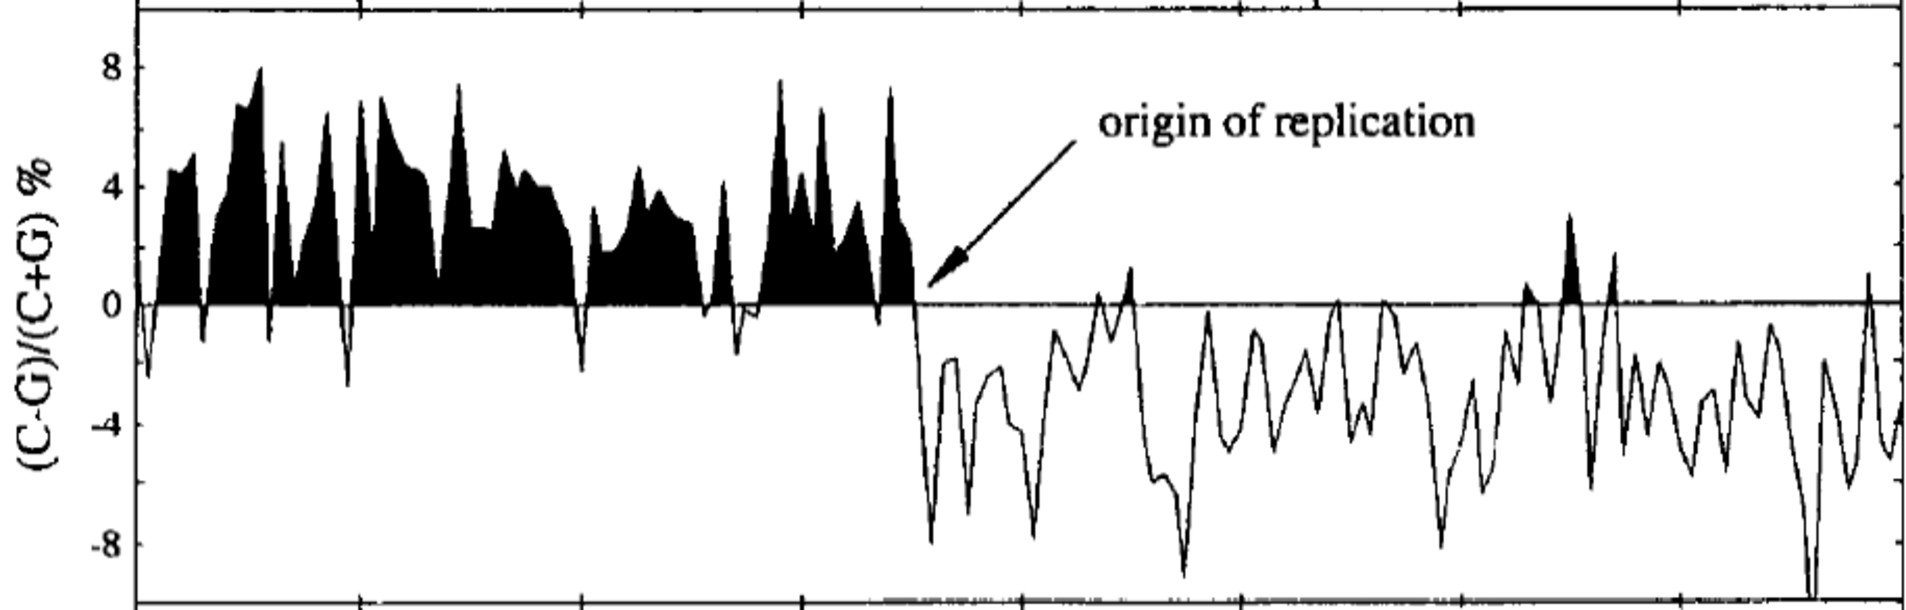
\includegraphics[width=\textwidth]{../figs/gcskewmbe96}
\caption{Screenshot of a part of figure 1 from \cite{LobryMBE96}.
  The GC-skew is computed in non-overlapping windows of 10 Kb
  along a 1.6 Mb fragment of the \textit{Escherichia coli}
  chromosome. The sequence is available with \texttt{data(m16j)}.}
\label{gcskewmbe96}
\end{minipage}
}
\end{figure}


The score here is the GC-skew computed in non-overlapping
windows of 10 Kb for a 1.6 Mb sequence.
We need a fragment of \textit{Escherchia coli} K12 chromosome from
67.4 min to 4.1 min on the genetic map\footnote{
The sequence is also directly available with \texttt{data(m16j)}.
}. Let's put this fragment into the string \texttt{myseq}:

\begin{Schunk}
\begin{Sinput}
 choosebank("greview")
 myseq1 <- gfrag("U00096", start = 3217270, length = 10^7)
 myseq2 <- gfrag("U00096", start = 1, length = 194133)
 closebank()
 myseq <- paste(myseq1, myseq2, sep = "")
 nchar(myseq)
\end{Sinput}
\begin{Soutput}
[1] 1616539
\end{Soutput}
\end{Schunk}

This is not exactly the same sequence that was used in \cite{LobryMBE96}
but very close to\footnote{
The sequence used in \cite{LobryMBE96} was a 1,616,174 bp fragment obtained
from the concatenation of nine overlapping sequences
(U18997, U00039, L10328, M87049, L19201, U00006, U14003, D10483, D26562
\cite{SofiaHJ1994, BurlandV1993, DanielsDL1992, PlunkettG1993, BlattnerFR1993, YuraT1992}).
Ambiguities have been resolved since then and its was a chimeric sequence
from K-12 strains MG1655 and W3110 \cite{HayashiK2006}, the sequence used here
is from strain MG1655 only \cite{BlattnerFR1997}. 
}. We define a function called \texttt{gcskew()} that computes our score 
for a given string \texttt{x}:

\begin{Schunk}
\begin{Sinput}
 gcskew <- function(x) {
     if (!is.character(x) || length(x) > 1) 
         stop("single string expected")
     tmp <- tolower(s2c(x))
     nC <- sum(tmp == "c")
     nG <- sum(tmp == "g")
     if (nC + nG == 0) 
         return(NA)
     return(100 * (nC - nG)/(nC + nG))
 }
 gcskew("GCCC")
\end{Sinput}
\begin{Soutput}
[1] 50
\end{Soutput}
\begin{Sinput}
 gcskew("GCCCNNNNNN")
\end{Sinput}
\begin{Soutput}
[1] 50
\end{Soutput}
\end{Schunk}

Note some defensive programming tricks used here:

\begin{itemize}
\item We check that the argument \texttt{x} is a single string.
\item We expand it as vector of single chars with \texttt{s2c()} only within the
      function to avoid big objects in the workspace.
\item We force to lower case letters with \texttt{tolower()} so that we can use 
      upper case letters too.
\item We avoid division by zero and return \texttt{NA} in this case.
\item We do not divide by the length of \texttt{x} but by the actual number
      of C and G so that ambiguous bases such as N do not introduce biases.
\end{itemize}


We move now along the sequence to compute the GC-skew:

\begin{Schunk}
\begin{Sinput}
 step <- 10000
 wsize <- 10000
 starts <- seq(from = 1, to = nchar(myseq), by = step)
 starts <- starts[-length(starts)]
 n <- length(starts)
 result <- numeric(n)
 for (i in seq_len(n)) {
     result[i] <- gcskew(substr(myseq, starts[i], starts[i] + 
         wsize - 1))
 }
\end{Sinput}
\end{Schunk}

The following code\footnote{
This code is adapted from the code at \url{http://www.stat.auckland.ac.nz/~paul/RGraphics/chapter3.html} for
figure 3.25 in Paul Murrell's book \cite{MurrellP2005}. This book is a must read if you are interested
by \Rlogo{}'s \textit{force de frappe} in the graphic domain. 
} was used to produce figure \ref{gcplot}.

\begin{Schunk}
\begin{Sinput}
 xx <- starts/1000
 yy <- result
 n <- length(result)
 hline <- 0
 plot(yy ~ xx, type = "n", axes = FALSE, ann = FALSE, ylim = c(-10, 
     10))
 polygon(c(xx[1], xx, xx[n]), c(min(yy), yy, min(yy)), col = "black", 
     border = NA)
 usr <- par("usr")
 rect(usr[1], usr[3], usr[2], hline, col = "white", border = NA)
 lines(xx, yy)
 abline(h = hline)
 box()
 axis(1, at = seq(0, 1600, by = 200))
 axis(2, las = 1)
 title(xlab = "position (Kbp)", ylab = "(C-G)/(C+G) %", main = expression(paste("GC skew in ", 
     italic(Escherichia ~ ~coli))))
 arrows(860, 5.5, 720, 0.5, length = 0.1, lwd = 2)
 text(860, 5.5, "origin of replication", pos = 4)
\end{Sinput}
\end{Schunk}

\begin{figure}
\centering\fbox{
\begin{minipage}{\textwidth}
\centering
\includegraphics[width=\textwidth]{../figs/FAQ-gcplot}
\caption{Re-creation of figure \ref{gcskewmbe96} from scratch.}
\label{gcplot}
\end{minipage}
}
\end{figure}

You can now play with the \texttt{wsize} and \texttt{step} parameters
to explore the signal (but note that with overlapping windows your
points are no more independent) or use all the smoothing tools
available under \Rlogo{}. Figure \ref{demolowess} shows for instance 
what can be obtained with the \texttt{lowess()} function with two
values for the smoothing parameter \texttt{f}. The corresponding code
is as follows:

\begin{Schunk}
\begin{Sinput}
 plot(xx, yy, col = "grey", type = "b", ylim = c(-10, 10), 
     las = 1, xaxt = "n", main = expression(paste("GC skew in ", 
         italic(Escherichia ~ ~coli))), xlab = "position (Kbp)", 
     ylab = "(C-G)/(C+G) %")
 axis(1, at = seq(0, 1600, by = 200))
 lines(smooth <- lowess(xx, yy, f = 0.05), lwd = 1)
 polycurve <- function(x, y, base.y = min(y), ...) polygon(x = c(min(x), 
     x, max(x)), y = c(base.y, y, base.y), ...)
 up <- smooth$y > 0
 polycurve(smooth$x[up], smooth$y[up], base.y = 0, col = rgb(0, 
     0, 1, 0.5))
 lines(lowess(xx, yy, f = 0.2), lwd = 2, col = "red")
 legend("topright", inset = 0.01, legend = c("f = 0.05", "f = 0.20"), 
     lwd = c(1, 2), col = c("black", "red"))
 abline(h = 0)
 arrows(860, 5.5, 720, 0.5, length = 0.1, lwd = 2)
 text(860, 5.5, "origin of replication", pos = 4)
\end{Sinput}
\end{Schunk}

\begin{figure}
\centering\fbox{
\begin{minipage}{\textwidth}
\centering
\includegraphics[width=\textwidth]{../figs/FAQ-demolowess}
\caption{Playing with the smoothing parameter \texttt{f} of
  the \texttt{lowess()} function.}
\label{demolowess}
\end{minipage}
}
\end{figure}


\section{How can I extract just a fragment from my sequence?}

Use the generic function \texttt{getFrag()} :

\begin{Schunk}
\begin{Sinput}
 choosebank("emblTP")
 query("mylist", "AC=A00001")
 getFrag(mylist$req[[1]], begin = 10, end = 20)
\end{Sinput}
\begin{Soutput}
[1] "gatggagaatt"
attr(,"seqMother")
[1] "A00001"
attr(,"begin")
[1] 10
attr(,"end")
[1] 20
attr(,"class")
[1] "SeqFrag"
\end{Soutput}
\begin{Sinput}
 closebank()
\end{Sinput}
\end{Schunk}

\section{How do I compute a score on my sequences?}

In the example below we want to compute the G+C content in third codon
positions for complete ribosomal CDS from \textit{Escherichia coli}:

\begin{Schunk}
\begin{Sinput}
 choosebank("emblTP")
 query("ecribo", "sp=escherichia coli ET t=cds ET k=ribosom@ ET NO k=partial")
 myseqs <- sapply(ecribo$req, getSequence)
 (gc3 <- sapply(myseqs, GC3))
\end{Sinput}
\begin{Soutput}
 [1] 0.4946237 0.6046512 0.5000000 0.6194030 0.5772727 0.4838710 0.5980066
 [8] 0.4974359 0.5031250 0.4324324 0.5000000 0.5113636 0.5290520 0.6142857
[15] 0.4904762 0.5714286 0.6191860 0.5906040 0.4880000 0.4880000 0.4946237
[22] 0.6046512 0.5000000 0.3522727 0.5076923 0.4343434 0.6194030 0.5522388
[29] 0.6104651 0.5661157 0.4946237 0.4946237 0.6079734 0.5000000 0.6343284
[36] 0.4659091 0.5789474 0.4946237 0.5000000 0.4974359 0.5689655 0.4611111
[43] 0.4611111 0.5303030 0.5303030 0.4482759 0.4201681 0.5915493 0.5000000
[50] 0.3829787 0.4519231 0.4302326 0.5696203 0.4285714 0.5689655 0.5000000
[57] 0.5224417 0.5661157 0.6057692 0.4444444 0.4659091 0.4130435 0.4946237
[64] 0.5661157 0.4946237 0.5680272
\end{Soutput}
\end{Schunk}

At the amino-acid level, we may get an estimate of the isoelectric point of
the proteins this way:

\begin{Schunk}
\begin{Sinput}
 sapply(sapply(myseqs, getTrans), computePI)
\end{Sinput}
\begin{Soutput}
 [1]  6.624309  7.801329 10.864793  5.931989  7.830476  6.624309  7.801329
 [8]  9.203410  9.826485  5.674672  7.154423  6.060457  6.313741  5.571446
[15]  9.435422  4.310747  6.145496  4.876054 11.006430 10.876036  6.624309
[22]  7.801329 10.864793  9.346289  9.203410  5.877050  5.931989  9.934988
[29]  5.920490  6.612505  6.624309  6.624309  7.801329 10.864793  5.931989
[36] 11.182499  9.598944  6.624309 10.864793  9.203410 11.031943  5.858421
[43]  5.858421 11.777511 11.777516 10.619175 11.365738  9.460987 10.864793
[50] 13.002381  9.845859 10.584868 11.421252 10.248325 11.031938 10.402075
[57]  4.863862  6.612505  9.681066 11.150304 11.182505 11.043607  6.624309
[64]  6.612505  6.624309  4.310747
\end{Soutput}
\end{Schunk}

Note that some pre-defined vectors to compute linear forms on sequences are
available in the \texttt{EXP} data.

As a matter of convenience, you may encapsulate the computation of your favorite score 
within a function this way:

\begin{Schunk}
\begin{Sinput}
 GC3m <- function(list, ind = 1:list$nelem) sapply(sapply(list$req[ind], 
     getSequence), GC3)
 GC3m(ecribo)
\end{Sinput}
\begin{Soutput}
 [1] 0.4946237 0.6046512 0.5000000 0.6194030 0.5772727 0.4838710 0.5980066
 [8] 0.4974359 0.5031250 0.4324324 0.5000000 0.5113636 0.5290520 0.6142857
[15] 0.4904762 0.5714286 0.6191860 0.5906040 0.4880000 0.4880000 0.4946237
[22] 0.6046512 0.5000000 0.3522727 0.5076923 0.4343434 0.6194030 0.5522388
[29] 0.6104651 0.5661157 0.4946237 0.4946237 0.6079734 0.5000000 0.6343284
[36] 0.4659091 0.5789474 0.4946237 0.5000000 0.4974359 0.5689655 0.4611111
[43] 0.4611111 0.5303030 0.5303030 0.4482759 0.4201681 0.5915493 0.5000000
[50] 0.3829787 0.4519231 0.4302326 0.5696203 0.4285714 0.5689655 0.5000000
[57] 0.5224417 0.5661157 0.6057692 0.4444444 0.4659091 0.4130435 0.4946237
[64] 0.5661157 0.4946237 0.5680272
\end{Soutput}
\begin{Sinput}
 GC3m(ecribo, 1:10)
\end{Sinput}
\begin{Soutput}
 [1] 0.4946237 0.6046512 0.5000000 0.6194030 0.5772727 0.4838710 0.5980066
 [8] 0.4974359 0.5031250 0.4324324
\end{Soutput}
\end{Schunk}

\section{Why do I have not exactly the same G+C content as in \texttt{codonW}?}

This question was raised (and solved) by Oliver Clay in an e-mail (23-AUG-2006).
The program \texttt{codonW} was written in C as part of John Peden's PhD thesis 
on Codon Usage \cite{codonW} and is available at \url{http://codonw.sourceforge.net/}.
The reason for the small differences in G+C content between the two programs is
that the default behavior in \texttt{codonW} is to remove the stop codon before
computations. Here is one way of removing the stop codon under \Rlogo{}:

\begin{Schunk}
\begin{Sinput}
 gc3nos <- sapply(myseqs, function(s) GC3(s[1:(length(s) - 
     3)]))
\end{Sinput}
\end{Schunk}

As compared with the previous result, the difference is small but visible:

\begin{Schunk}
\begin{Sinput}
 plot(x = gc3, y = gc3nos, las = 1, main = "Stop codon removal effect on G+C content\nin third codon positions", 
     xlab = "With stop codon", ylab = "Stop codons removed")
 abline(c(0, 1))
\end{Sinput}
\end{Schunk}
\includegraphics{../figs/FAQ-stopcodonremovaleffect}

\texttt{CodonW} was released with a test file called \texttt{input.dat}, here are
the first 10 lines of the file copied from \texttt{CodonWSourceCode\_1\_4\_4}:

\begin{Schunk}
\begin{Sinput}
 inputdatfile <- system.file("sequences/input.dat", package = "seqinr")
 cat(readLines(inputdatfile, n = 10), sep = "\n")
\end{Sinput}
\begin{Soutput}
>YCG9 Probable          1377 residues Pha 0 Code 0
ATGAATATGCTCATTGTCGGTAGAGTTGTTGCTAGTGTTGGGGGAAGCGGACTTCAAACG
CTTTGCTTTGTTATTGGTTGTACGATGGTTGGTGAAAGGTCACGTCCATTGGTGATTTCC
ATCCTAAGTTGTGCATTTGCTGTAGCTGCTATCGTTGGTCCTATAATCGGAGGTGCCTTT
ACAACCCATGTTACCTGGAGGTGGTGCTTCTATATCAATCTTCCTATCGGTGGTCTTGCC
ATTATTATGTTTTTACTCACATATAAGGCCGAGAATAAGGGTATACTTCAACAAATTAAA
GATGCTATAGGAACAATCTCGAGCTTTACTTTTAGTAAGTTCAGACACCAAGTTAATTTT
AAAAGACTTATGAATGGCATAATCTTCAAGTTTGACTTCTTTGGTTTTGCCCTCTGCTCT
GCAGGGCTGGTCCTTTTCCTACTGGGGCTAACCTTTGGTGGTAATAAATATAGTTGGAAC
TCTGGCCAAGTCATCGCATATTTGGTTTTGGGTGTCTTACTTTTTATTTTTTCATTGGTG
\end{Soutput}
\end{Schunk}

This is a FASTA file that we import under \Rlogo{}~with:

\begin{Schunk}
\begin{Sinput}
 input <- read.fasta(file = inputdatfile)
 names(input)
\end{Sinput}
\begin{Soutput}
  [1] "YCG9"      "YCG8"      "ALPHA2"    "ALPHA1"    "CHA1"      "KRR1"     
  [7] "PRD1"      "KAR4"      "PBN1"      "LRE1"      "APA1"      "YCE9"     
 [13] "YCE8"      "YCE7"      "YCE5"      "YCE6"      "YCE4"      "PDI1"     
 [19] "GLK1"      "YCD8"      "SRO9"      "YCD6"      "YCD5"      "YCD3"     
 [25] "STE50"     "HIS4"      "BIK1"      "FUS1"      "YC08"      "AGP1"     
 [31] "LEU2"      "NFS1"      "BUD3"      "GBP2"      "ILV6"      "CWH36"    
 [37] "PEL1"      "RER1"      "CDC10"     "MRPL32"    "YCP4"      "CIT2"     
 [43] "YCP7"      "SAT4"      "RVS161"    "YCQ0"      "ADP1"      "PGK1"     
 [49] "POL4"      "YCQ7"      "SRD1"      "MAK32"     "PET18"     "MAK31"    
 [55] "HSP30"     "YCR3"      "SYN"       "YCR6"      "GNS1"      "FEN2"     
 [61] "RIM1"      "CRY1"      "YCS2"      "YCS3"      "GNS1"      "RBK1"     
 [67] "PHO87"     "BUD5"      "MATALPHA2" "MATALPHA1" "TSM1"      "YCT5"     
 [73] "PETCR46"   "YCT7"      "YCT9"      "ARE1"      "RSC6"      "THR4"     
 [79] "CTR86"     "PWP2"      "YCU9"      "YCV1"      "G10"       "HCM1"     
 [85] "RAD18"     "CYPR"      "YCW1"      "YCW2"      "SSK22"     "SOL2"     
 [91] "ERS1"      "PAT1"      "SRB8"      "YCX3"      "TUP1"      "YC16"     
 [97] "ABP1"      "KIN82"     "MSH3"      "CDC39"     "YCY4"      "A2"       
[103] "GIT1"      "YCZ0"      "YCZ1"      "YCZ2"      "YCZ3"      "PAU3"     
[109] "YCZ5"      "YCZ6"      "YCZ7"     
\end{Soutput}
\end{Schunk}

The file \texttt{input.out} contains the values obtained with \texttt{codonW}
for the GC content and GC3s content:

\begin{Schunk}
\begin{Sinput}
 inputoutfile <- system.file("sequences/input.out", package = "seqinr")
 cat(readLines(inputoutfile, n = 10), sep = "\n")
\end{Sinput}
\begin{Soutput}
title                    	GC3s	GC	
YCG9_Probable__________13	0.335	0.394	
YCG8________573_residues_	0.439	0.446	
ALPHA2________633_residue	0.328	0.351	
ALPHA1________528_residue	0.345	0.379	
CHA1_________1083_residue	0.328	0.394	
KRR1__________951_residue	0.364	0.384	
PRD1_________2139_residue	0.430	0.397	
KAR4_________1008_residue	0.354	0.383	
PBN1_________1251_residue	0.330	0.386	
\end{Soutput}
\begin{Sinput}
 input.res <- read.table(inputoutfile, header = TRUE)
 head(input.res)
\end{Sinput}
\begin{Soutput}
                      title  GC3s    GC
1 YCG9_Probable__________13 0.335 0.394
2 YCG8________573_residues_ 0.439 0.446
3 ALPHA2________633_residue 0.328 0.351
4 ALPHA1________528_residue 0.345 0.379
5 CHA1_________1083_residue 0.328 0.394
6 KRR1__________951_residue 0.364 0.384
\end{Soutput}
\end{Schunk}

Let's try to reproduce the results for the G+C content, we know that we have to
remove the last stop codon:

\begin{Schunk}
\begin{Sinput}
 input.gc <- sapply(input, function(s) GC(s[1:(length(s) - 
     3)]))
 max(abs(input.gc - input.res$GC))
\end{Sinput}
\begin{Soutput}
[1] 0.0004946237
\end{Soutput}
\begin{Sinput}
 plot(x = input.gc, y = input.res$GC, las = 1, xlab = "Results with GC()", 
     ylab = "Results from codonW", main = "Comparison of G+C content results")
 abline(c(0, 1))
\end{Sinput}
\end{Schunk}
\includegraphics{../figs/FAQ-inputgc}

The results are consistent if we consider that we have 3 significant digits
in the file \texttt{input.out}. Now, let's try to reproduce the results
for G+C in third codon positions:

\begin{Schunk}
\begin{Sinput}
 input.gc3 <- sapply(input, function(s) GC3(s[1:(length(s) - 
     3)]))
 max(abs(input.gc3 - input.res$GC3s))
\end{Sinput}
\begin{Soutput}
[1] 0.054
\end{Soutput}
\begin{Sinput}
 plot(x = input.gc3, y = input.res$GC3s, las = 1, xlab = "Results with GC3()", 
     ylab = "Results from codonW", main = "Comparison of G+C content in third codon positions results")
 abline(c(0, 1))
\end{Sinput}
\end{Schunk}
\includegraphics{../figs/FAQ-inputgc3}

There is clearly a problem here. Looking into the documentation of
\texttt{codonW}, GC3s is the G+C content in third codon position
after removing non-synonymous and stop codons (those corresponding to Met, Trp, Stp).
Let's remove these codons:

\begin{Schunk}
\begin{Sinput}
 codons <- words()
 names(codons) <- sapply(codons, function(c) aaa(translate(s2c(c), 
     numcode = 1)))
 okcodons <- codons[!names(codons) %in% c("Met", "Trp", "Stp")]
 gc3s <- function(s) {
     tmp <- splitseq(s)
     tmp <- tmp[tmp %in% okcodons]
     tmp <- s2c(paste(tmp, collapse = ""))
     GC3(tmp)
 }
 input.gc3s <- sapply(input, gc3s)
 max(abs(input.gc3s - input.res$GC3s))
\end{Sinput}
\begin{Soutput}
[1] 0.0004980843
\end{Soutput}
\begin{Sinput}
 plot(x = input.gc3s, y = input.res$GC3s, las = 1, xlab = "Results with GC3()", 
     ylab = "Results from codonW", main = "Comparison of G+C content in third codon positions results\n(Met, Trp and Stp codons excluded)")
 abline(c(0, 1))
\end{Sinput}
\end{Schunk}
\includegraphics{../figs/FAQ-inputgc3s}

The results are now consistent. But thinking more about it there is still a problem
with the codons for Ile:

\begin{Schunk}
\begin{Sinput}
 codons[names(codons) == "Ile"]
\end{Sinput}
\begin{Soutput}
  Ile   Ile   Ile 
"ata" "atc" "att" 
\end{Soutput}
\end{Schunk}

There are three codons for Ile. If the distribution of the four bases was uniform and selectively
neutral in third codon position of synonymous codons, then we would expect to
get a G+C of 50\% in quartet and duet codons at third codons positions because they
all have the same number of W (A or T )and S (C or G) bases in third position. But for Ile 
we have two codons ending in W versus only one in S so that we would get a G+C
of $\frac{1}{3}$ instead of $\frac{1}{2}$. This point was clearly stated 
\cite{noboru88} by Sueoka in 1988:

\begin{quote}
\textbf{G + C Content of the Three Codons Positions.}
In the present analysis, observed G + C contents of the first, second, and third
codon positions ($P_{1}$, $P_{2}$, and $P_{3}$, respectively) are corrected
average G + C contents of the three codon positions that are calculated from
56 triplets out of 64. Because of the inequality of $\alpha$ and $\gamma$ at the
third codon position, the three stop codons (TAA, TAG, and TGA) and the three
codons for isoleucine (ATT, ATC, and ATA) were excluded in calculation of
$P_{3}$, and two single codons for methionine (ATG) and tryptophan (TGG)
were excluded in all three ($P_{1}$, $P_{2}$, and $P_{3}$)
\end{quote}

Let's compute $P_{3}$ and compare it with GC3s:

\begin{Schunk}
\begin{Sinput}
 P3codons <- codons[!names(codons) %in% c("Met", "Trp", "Ile", 
     "Stp")]
 P3 <- function(s) {
     tmp <- splitseq(s)
     tmp <- tmp[tmp %in% P3codons]
     tmp <- s2c(paste(tmp, collapse = ""))
     GC3(tmp)
 }
 input.P3 <- sapply(input, P3)
 max(abs(input.P3 - input.res$GC3s))
\end{Sinput}
\begin{Soutput}
[1] 0.02821505
\end{Soutput}
\begin{Sinput}
 plot(x = input.P3, y = input.res$GC3s, las = 1, xlab = "Results with P3", 
     ylab = "Results from codonW GC3s", main = "Comparison of P3 and GC3s")
 abline(c(0, 1))
\end{Sinput}
\end{Schunk}
\includegraphics{../figs/FAQ-inputP3}

This is not exactly the same, the maximum observed difference here is about $3\%$.
In practice, $P_{3}$, GC3, and GC3s are only slightly different \cite{noboru99}.

\section{How do I get a sequence from its name?}

This question is adapted from an e-mail (22 Jun 2006) by Gang Xu.
I know that the UniProt (SwissProt) entry of my protein is \texttt{P08758},
if I know its name\footnote{
More exactly, this is the accession number. Sequence names are not stable over time,
it's always better to use the accession numbers. 
}, how can I get the sequence?

\begin{Schunk}
\begin{Sinput}
 choosebank("swissprot")
 query("myprot", "AC=P08758")
 getSequence(myprot$req[[1]])
\end{Sinput}
\begin{Soutput}
  [1] "M" "A" "Q" "V" "L" "R" "G" "T" "V" "T" "D" "F" "P" "G" "F" "D" "E" "R"
 [19] "A" "D" "A" "E" "T" "L" "R" "K" "A" "M" "K" "G" "L" "G" "T" "D" "E" "E"
 [37] "S" "I" "L" "T" "L" "L" "T" "S" "R" "S" "N" "A" "Q" "R" "Q" "E" "I" "S"
 [55] "A" "A" "F" "K" "T" "L" "F" "G" "R" "D" "L" "L" "D" "D" "L" "K" "S" "E"
 [73] "L" "T" "G" "K" "F" "E" "K" "L" "I" "V" "A" "L" "M" "K" "P" "S" "R" "L"
 [91] "Y" "D" "A" "Y" "E" "L" "K" "H" "A" "L" "K" "G" "A" "G" "T" "N" "E" "K"
[109] "V" "L" "T" "E" "I" "I" "A" "S" "R" "T" "P" "E" "E" "L" "R" "A" "I" "K"
[127] "Q" "V" "Y" "E" "E" "E" "Y" "G" "S" "S" "L" "E" "D" "D" "V" "V" "G" "D"
[145] "T" "S" "G" "Y" "Y" "Q" "R" "M" "L" "V" "V" "L" "L" "Q" "A" "N" "R" "D"
[163] "P" "D" "A" "G" "I" "D" "E" "A" "Q" "V" "E" "Q" "D" "A" "Q" "A" "L" "F"
[181] "Q" "A" "G" "E" "L" "K" "W" "G" "T" "D" "E" "E" "K" "F" "I" "T" "I" "F"
[199] "G" "T" "R" "S" "V" "S" "H" "L" "R" "K" "V" "F" "D" "K" "Y" "M" "T" "I"
[217] "S" "G" "F" "Q" "I" "E" "E" "T" "I" "D" "R" "E" "T" "S" "G" "N" "L" "E"
[235] "Q" "L" "L" "L" "A" "V" "V" "K" "S" "I" "R" "S" "I" "P" "A" "Y" "L" "A"
[253] "E" "T" "L" "Y" "Y" "A" "M" "K" "G" "A" "G" "T" "D" "D" "H" "T" "L" "I"
[271] "R" "V" "M" "V" "S" "R" "S" "E" "I" "D" "L" "F" "N" "I" "R" "K" "E" "F"
[289] "R" "K" "N" "F" "A" "T" "S" "L" "Y" "S" "M" "I" "K" "G" "D" "T" "S" "G"
[307] "D" "Y" "K" "K" "A" "L" "L" "L" "L" "C" "G" "E" "D" "D"
\end{Soutput}
\end{Schunk}


\section*{Session Informations}

\begin{scriptsize}

This part was compiled under the following \Rlogo{}~environment:

\begin{itemize}
  \item R version 2.9.0 (2009-04-17), \verb|i386-apple-darwin8.11.1|
  \item Locale: \verb|fr_FR.UTF-8/fr_FR.UTF-8/fr_FR.UTF-8/C/C/C|
  \item Base packages: base, datasets, graphics, grDevices, grid,
    methods, stats, utils
  \item Other packages: ade4~1.4-11, ape~2.3, grImport~0.4-3,
    MASS~7.2-46, quadprog~1.4-11, seqinr~2.0-3, tseries~0.10-18,
    XML~2.3-0, xtable~1.5-5, zoo~1.5-5
  \item Loaded via a namespace (and not attached): gee~4.13-13,
    lattice~0.17-22, nlme~3.1-90
\end{itemize}
There were two compilation steps:

\begin{itemize}
  \item \Rlogo{} compilation time was: Thu Apr 23 12:57:33 2009
  \item \LaTeX{} compilation time was: \today
\end{itemize}

\end{scriptsize}

% END - DO NOT REMOVE THIS LINE

%%%%%%%%%%%%  BIBLIOGRAPHY %%%%%%%%%%%%%%%%%
\clearpage
\addcontentsline{toc}{section}{References}
\bibliographystyle{plain}
\bibliography{../config/book}
\end{document}
